% Compile with: xelatex final_report.tex
% If compiling from the project root, use:
% xelatex -output-directory=report report/final_report.tex
\documentclass[UTF8,a4paper,12pt]{ctexart}

\usepackage{geometry}
\usepackage{graphicx}
\usepackage{booktabs}
\usepackage{float}
\usepackage{amsmath}
\usepackage{hyperref}
\usepackage{array}
\usepackage{xcolor}

\geometry{left=2.6cm,right=2.6cm,top=2.5cm,bottom=2.5cm}
\graphicspath{{report/figures/}{figures/}{experiments/figures/}{../experiments/figures/}}
\hypersetup{
  colorlinks=true,
  linkcolor=blue,
  urlcolor=blue,
  citecolor=blue
}

\title{家庭用电多变量时间序列预测实验报告}
\author{请填写姓名、学号与班级}
\date{\today}

\begin{document}
\maketitle

\begin{abstract}
本实验面向家庭用电多变量时间序列预测任务，使用过去 90 天的每日用电和天气特征，分别预测未来 90 天和未来 365 天的总有功功率曲线。实验比较 LSTM、Transformer 和本文提出的 CNN+Transformer 改进模型。每个模型在两个预测任务上均使用 5 个随机种子独立训练，并以测试集反标准化后的 MSE 和 MAE 作为主要指标。实验结果显示，CNN+Transformer 在 90 天预测和 365 天预测中均取得最低平均误差，说明局部卷积特征与全局注意力机制的结合对该任务具有较好效果。
\end{abstract}

\noindent
代码仓库链接：\url{https://github.com/Haemonculus-WH40k/ML_final_2026.git}

\section{问题介绍}

本项目研究家庭用电多变量时间序列预测问题。原始用电数据来自 UCI Individual household electric power consumption 数据集，记录了 2006-12-16 17:24:00 至 2010-11-26 21:02:00 期间的分钟级家庭用电信息。主要原始字段包括总有功功率、总无功功率、电压、电流强度以及三个分表能耗。

课程任务要求基于过去 90 天的数据曲线预测未来用电曲线。本项目完成两个独立预测任务：

\begin{itemize}
  \item 短期预测：输入过去 90 天，预测未来 90 天；
  \item 长期预测：输入过去 90 天，预测未来 365 天。
\end{itemize}

两个任务分别训练模型，长期预测模型不复用短期预测模型参数。实验比较三种方法：LSTM、Transformer 和 CNN+Transformer 改进模型。评估指标为 MSE 和 MAE，每个模型、每个预测长度均进行 5 轮独立实验，并报告均值与标准差。

\subsection*{数据清洗与特征构造}

原始分钟级数据中缺失值使用问号表示。预处理流程如下：

\begin{enumerate}
  \item 合并 \texttt{Date} 和 \texttt{Time} 为统一时间戳；
  \item 将问号转换为缺失值，并将数值列转换为浮点数；
  \item 按分钟重建完整时间索引，对缺失分钟进行时间插值和双向填充；
  \item 计算剩余分表能耗：
\end{enumerate}

\begin{equation}
\texttt{sub\_metering\_remainder}
= \texttt{global\_active\_power} \times \frac{1000}{60}
- \texttt{sub\_metering\_1}
- \texttt{sub\_metering\_2}
- \texttt{sub\_metering\_3}.
\end{equation}

随后将分钟级数据聚合为每日数据。其中功率和分表能耗相关字段按天求和，电压和电流强度按天求平均。处理后得到 1441 天每日数据，日期范围为 2006-12-17 至 2010-11-26。

天气数据使用法国 Hauts-de-Seine 省，省编号 92，月度基础气象数据文件为 \texttt{MENSQ\_92\_previous-1950-2024.csv.gz}。使用的天气字段包括 \texttt{RR}、\texttt{NBJRR1}、\texttt{NBJRR5}、\texttt{NBJRR10} 和 \texttt{NBJBROU}。其中 \texttt{RR} 按课程要求除以 10，多个气象站同月记录按字段取平均值，并按月份合并到每日用电数据中。

最终建模特征共 13 个，包括 8 个用电特征和 5 个天气特征。目标变量为每日 \texttt{global\_active\_power}。由于课程提到的 \texttt{train.csv} 和 \texttt{tes.csv/test.csv} 当前未在项目目录中提供，本项目按时间顺序划分窗口样本，训练集、验证集、测试集比例为 70\%、15\%、15\%。标准化参数仅在训练段拟合，再应用于验证集和测试集，以避免未来信息泄漏。

\section{模型}

本项目实现三种模型。三种方法均接收形状为 $[B, 90, F]$ 的输入，其中 $B$ 为 batch size，$F=13$ 为特征数。模型输出为未来 $H$ 天的目标序列，短期任务 $H=90$，长期任务 $H=365$。

\subsection{LSTM 模型}

LSTM 是循环神经网络模型，适合处理有序序列。本文使用多层 LSTM 编码过去 90 天的多变量输入，取最后一个时间步的隐状态作为历史窗口表示，再通过 LayerNorm、Dropout 和全连接层直接输出未来序列。

\begin{verbatim}
Input: X in R^{B x 90 x F}
h_1, ..., h_90 = LSTM(X)
z = h_90
y_hat = Linear(Dropout(LayerNorm(z)))
Output: y_hat in R^{B x H}
\end{verbatim}

LSTM 作为基础循环模型，可以捕捉时间顺序信息，但在较长预测跨度下容易受到隐藏状态容量限制。

\subsection{Transformer 模型}

Transformer 通过自注意力机制建模序列内部任意位置之间的依赖关系。本文首先使用线性层将输入特征映射到 \texttt{d\_model} 维空间，再加入正弦位置编码，然后通过 Transformer Encoder 建模 90 天历史序列。最后对时间维做平均池化，并通过全连接预测头输出未来曲线。

\begin{verbatim}
Input: X in R^{B x 90 x F}
E = Linear(X) + PositionalEncoding
Z = TransformerEncoder(E)
z = MeanPooling(Z, time dimension)
y_hat = Linear(LayerNorm(z))
Output: y_hat in R^{B x H}
\end{verbatim}

Transformer 的优势在于全局依赖建模能力较强，但在样本规模较小时容易出现过拟合或对局部波动建模不足的问题。

\subsection{CNN+Transformer 改进模型}

本文提出的改进模型先使用一维卷积提取局部用电模式，再使用 Transformer Encoder 建模全局时间依赖。卷积层可以捕捉短期波动、尖峰和局部周期，Transformer 则负责建模 90 天窗口中的长依赖关系。

\begin{verbatim}
Input: X in R^{B x 90 x F}
X_c = Transpose(X)                 # B x F x 90
C = Conv1D + GELU + BatchNorm + Conv1D + GELU
E = Transpose(C) + PositionalEncoding
Z = TransformerEncoder(E)
z = LastState(Z) or MeanPooling(Z)
y_hat = MLP(z)
Output: y_hat in R^{B x H}
\end{verbatim}

该模型的核心思想是将局部模式提取和全局依赖建模结合起来。与单纯 LSTM 相比，它不依赖单一递归隐藏状态；与单纯 Transformer 相比，它在进入自注意力模块前先强化了局部时序结构。

\section{结果与分析}

\subsection*{实验设置}

正式实验统一配置如下：

\begin{itemize}
  \item 随机种子：42、2026、7、13、99；
  \item 最大 epoch：100；
  \item early stopping patience：10；
  \item batch size：64；
  \item optimizer：AdamW；
  \item learning rate：0.001；
  \item weight decay：0.0001；
  \item loss：MSELoss。
\end{itemize}

每个模型在短期和长期任务上各运行 5 次，共 30 次正式训练。训练过程保存标准化空间预测结果，并反标准化回 \texttt{global\_active\_power} 原始单位后计算最终 MSE 和 MAE。

\subsection*{结果表}

表 \ref{tab:summary} 给出测试集反标准化后的汇总指标。图 \ref{fig:summary-shot} 为由实验结果文件生成的结果截图。

\begin{table}[H]
\centering
\caption{三种方法在两个预测任务上的测试集结果}
\label{tab:summary}
\small
\begin{tabular}{llrrrr}
\toprule
任务 & 模型 & MSE Mean & MSE Std & MAE Mean & MAE Std \\
\midrule
90 天预测 & LSTM & 287850.41 & 5995.96 & 429.60 & 5.29 \\
90 天预测 & Transformer & 292620.39 & 25074.70 & 439.39 & 22.79 \\
90 天预测 & CNN+Transformer & 212555.30 & 30997.75 & 362.90 & 30.66 \\
365 天预测 & LSTM & 190709.40 & 16130.92 & 337.09 & 17.03 \\
365 天预测 & Transformer & 178740.92 & 17516.37 & 325.48 & 18.32 \\
365 天预测 & CNN+Transformer & 165483.01 & 12328.18 & 310.95 & 13.41 \\
\bottomrule
\end{tabular}
\end{table}

\begin{figure}[H]
\centering
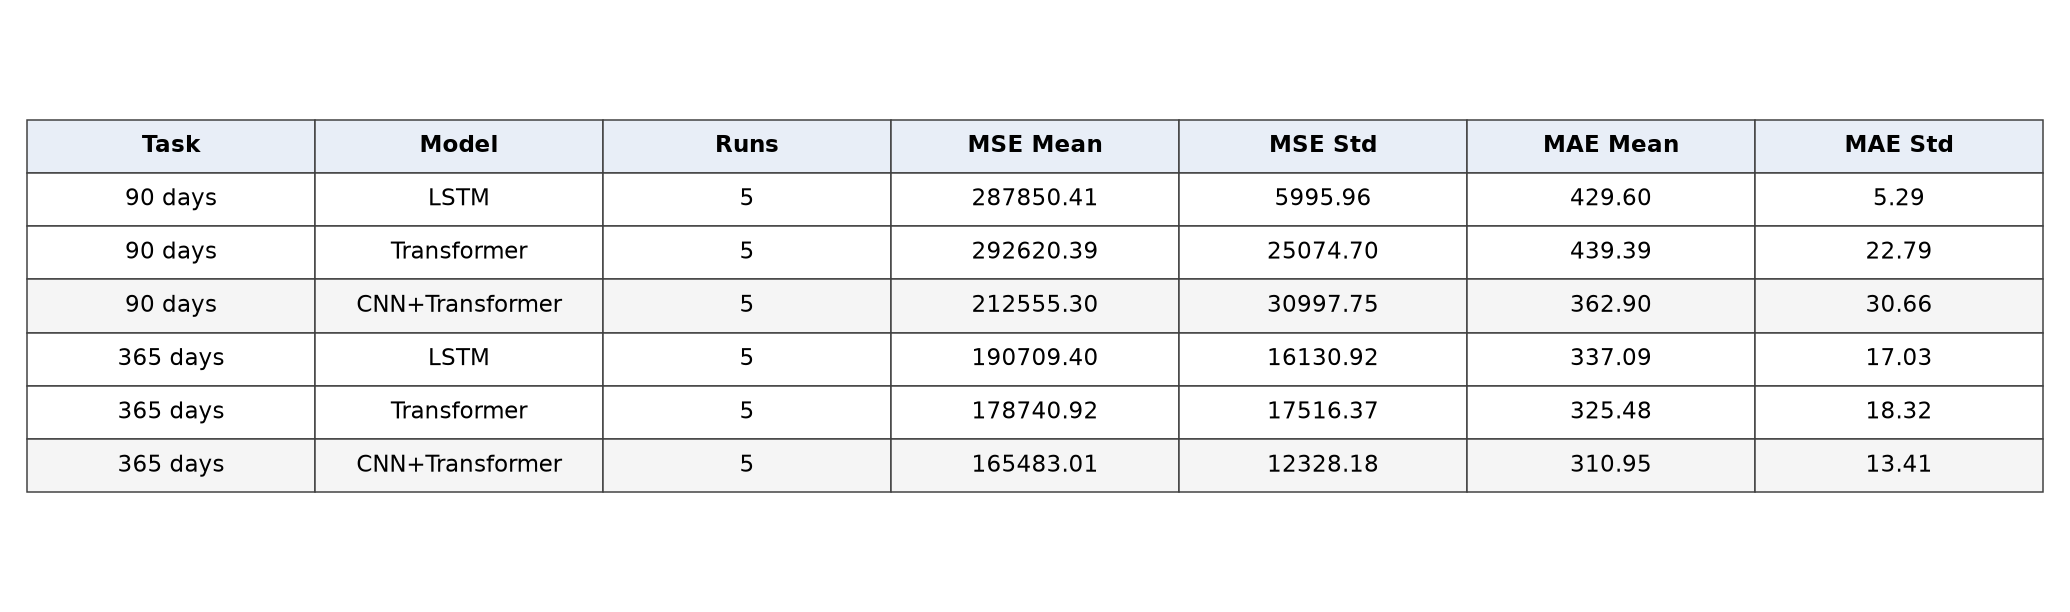
\includegraphics[width=\textwidth]{summary_table_screenshot.png}
\caption{实验结果截图：三种方法在短期和长期预测任务上的 MSE、MAE 均值与标准差。}
\label{fig:summary-shot}
\end{figure}

\subsection*{预测曲线对比}

图 \ref{fig:short-curve} 和图 \ref{fig:long-curve} 分别展示 90 天预测和 365 天预测中，同一测试样本上三种方法的预测曲线与 Ground Truth 曲线对比。

\begin{figure}[H]
\centering
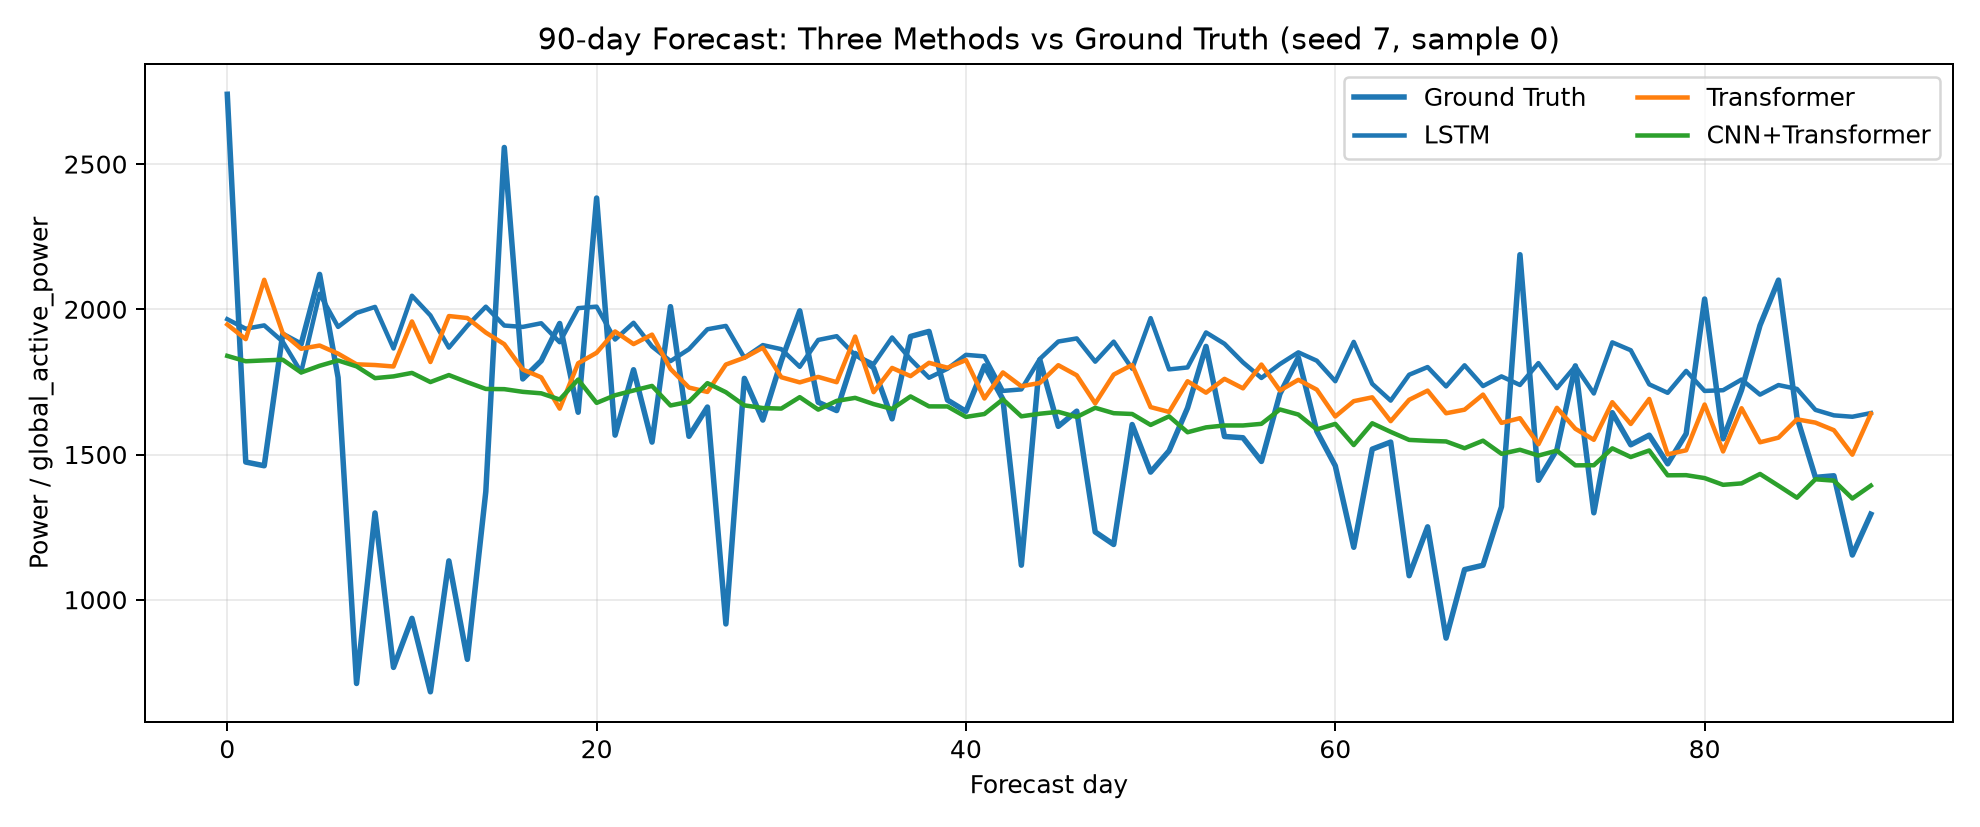
\includegraphics[width=\textwidth]{short_three_methods_vs_gt.png}
\caption{90 天预测任务中三种方法与 Ground Truth 的电量曲线对比。}
\label{fig:short-curve}
\end{figure}

\begin{figure}[H]
\centering
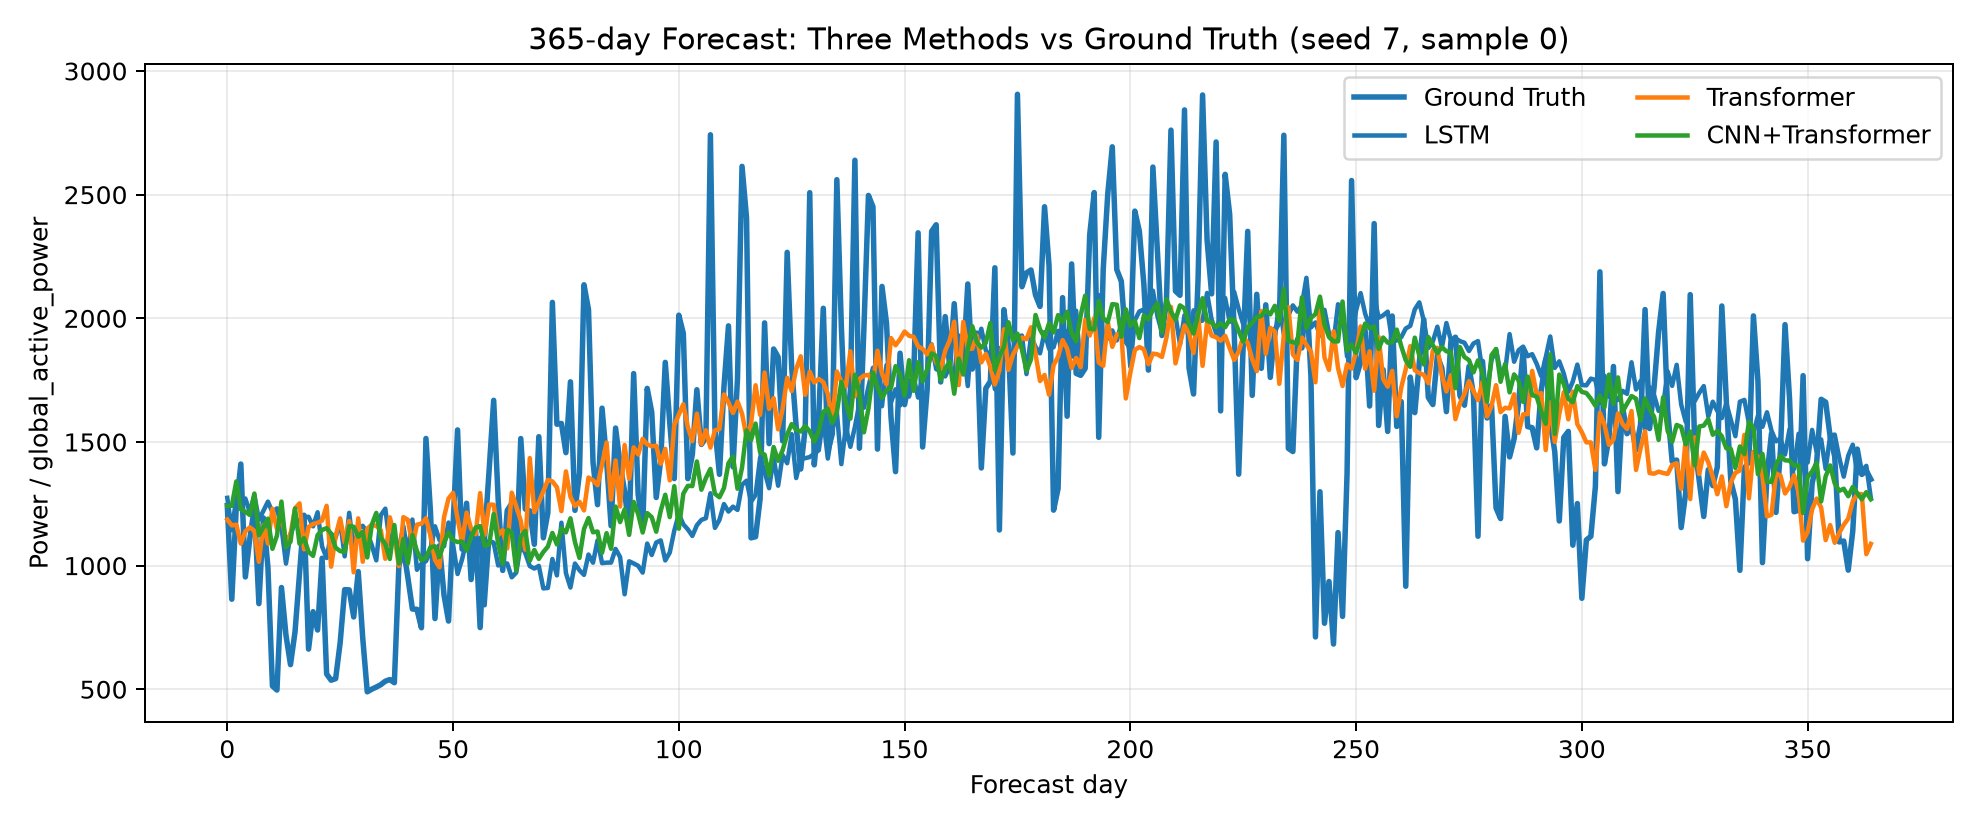
\includegraphics[width=\textwidth]{long_three_methods_vs_gt.png}
\caption{365 天预测任务中三种方法与 Ground Truth 的电量曲线对比。}
\label{fig:long-curve}
\end{figure}

\subsection*{三种方法比较}

从表 \ref{tab:summary} 可以看出，在 90 天预测任务中，CNN+Transformer 的平均 MSE 为 212555.30，平均 MAE 为 362.90，均低于 LSTM 和 Transformer。这说明在短期预测中，先通过卷积提取局部用电模式能够有效改善预测效果。LSTM 在短期任务中的 MAE 标准差较小，说明结果较稳定，但平均误差明显高于改进模型。Transformer 的短期结果略弱，可能与样本规模有限、自注意力模型较依赖数据量有关。

在 365 天预测任务中，Transformer 的平均误差优于 LSTM，说明自注意力机制在较长预测跨度下比循环模型更有优势。CNN+Transformer 进一步将平均 MSE 降低到 165483.01，平均 MAE 降低到 310.95，并且 MAE 标准差也低于另外两种方法，说明改进模型在长期任务中同时具有较好的精度和稳定性。

从曲线形态看，三种模型都更容易学习到整体趋势和平均水平，但对短期尖峰、突然下降和高频波动的追踪仍有限。CNN+Transformer 的预测曲线整体更加平滑，但在平均误差上表现更优，说明该模型更好地把握了测试集中的主导趋势。

\section{讨论}

本实验完成了课程要求的两种预测任务和三类方法比较，并给出了每个模型、每个任务 5 轮实验的均值与标准差。总体来看，CNN+Transformer 在短期和长期任务上均取得最佳平均表现，验证了局部卷积特征与全局注意力机制结合的有效性。

但是，本项目仍存在一些限制。首先，原始用电数据只来自一个家庭，样本量有限，模型泛化能力仍需在更多家庭或更长时间跨度数据上验证。其次，天气数据为月度、省级聚合数据，不能反映每日温度、湿度、节假日和异常天气等细粒度因素，因此天气特征对日级预测的帮助可能有限。第三，当前模型均采用一次性多步输出方式，没有显式建模未来输出序列之间的自回归依赖，因此对突发峰值和快速变化的预测能力不足。

后续可以从以下方向改进：

\begin{itemize}
  \item 引入日级或小时级天气数据，提高外部变量的时间分辨率；
  \item 加入星期、月份、节假日等时间特征；
  \item 使用趋势项、周期项和残差项分解后分别建模；
  \item 对 CNN+Transformer 进行更系统的超参数搜索；
  \item 分析预测误差较大的样本，针对峰值和异常波动设计专门损失函数或模型结构。
\end{itemize}

本项目代码和实验产物已上传至 GitHub：\url{https://github.com/Haemonculus-WH40k/ML_final_2026.git}。正式提交前，请根据课程要求补充作者姓名、学号、组员贡献和必要的参考文献格式。

\end{document}
